\subsection{Recursion}

\begin{frame}[fragile]
\frametitle{Recursion}
\begin{figure}[h]
\centering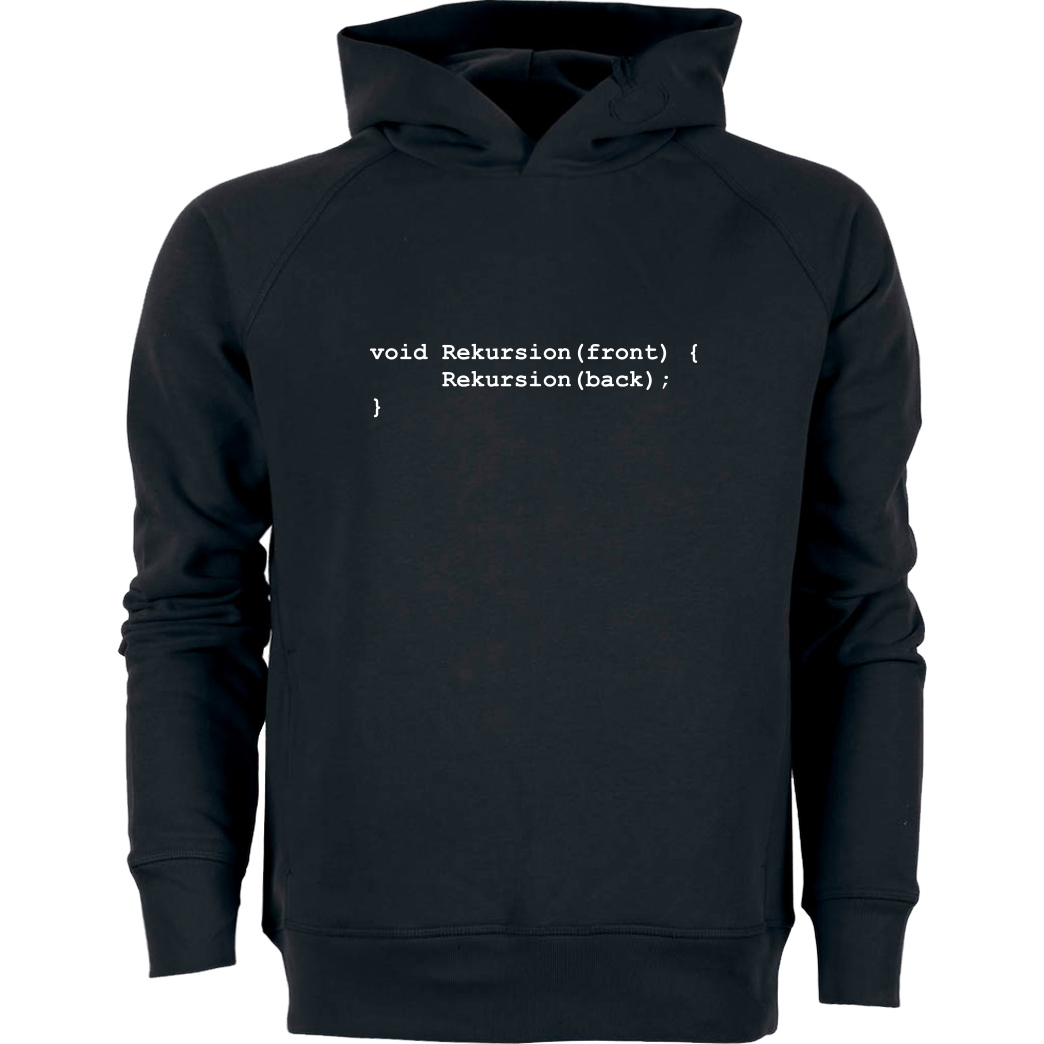
\includegraphics[scale=0.15]{img/recursion.jpg}
\caption{Recursion}
\end{figure}
\end{frame}

\begin{frame}[fragile]
\frametitle{Factorial}

\begin{definition}[Factorial]
\begin{align}
n! = 1 \cdot 2 \cdot ... \cdot (n-1) \cdot n
\end{align}
\end{definition}

\begin{definition}[Factorial Recursive]
\begin{align}
n!=\left\{\begin{aligned} & 1 & & n=0\\
& n \cdot (n-1)! & & n>0 \end{aligned}\right.
\end{align}
\end{definition}
\end{frame}

\begin{frame}[fragile]
\frametitle{Factorial}
{\tiny
\lstinputlisting{code/rekursion/fakultaet.cpp}
}
Runtime: $O(n)$
\end{frame}

\begin{frame}[fragile]
\frametitle{Factorial - Exercise}
\begin{exercise}
What is the biggest number for which the factorial could be calculated (under usage
of the code above)?
\end{exercise}
\end{frame}

\begin{frame}[fragile]
\frametitle{Fibonacci Numbers}
\begin{definition}[Fibonacci Zahlen]
\begin{align}
F_n=\left\{
\begin{aligned} & 0 & & n=0\\
& 1 & & n=1\\
& F_{n-1} + F_{n-2} & & n>1
\end{aligned}\right.
\end{align}
\end{definition}
\end{frame}

\begin{frame}[fragile]
\frametitle{Fibonacci Numbers}
{\tiny
\lstinputlisting{code/rekursion/fibonacci.cpp}
}
\end{frame}

\begin{frame}[fragile]
\frametitle{Fibonacci Numbers - Exercise}
\begin{exercise}
Rewrite the recursive function for calculating the fibonacci numbers to an iterative
version. Which one is faster, recursive or iterative?
\end{exercise}
\end{frame}

\begin{frame}[fragile]
\frametitle{Power}

\begin{definition}[Power]
\begin{align}
a^n = \underbrace{a \cdot a \cdot a \cdot ... \cdot a}_\text{n factors}
\end{align}
\end{definition}

\begin{definition}[Power Recursive]
\begin{align}
a^n=\left\{\begin{aligned} & a^{\frac{n}{2}} \cdot a^{\frac{n}{2}} & & \text{n even}\\
& a^{\frac{n-1}{2}} \cdot a^{\frac{n-1}{2}} \cdot a & & \text{n odd} \end{aligned}\right.
\end{align}
\end{definition}

\end{frame}

\begin{frame}[fragile]
\frametitle{Power - Iterative}
{\tiny
\lstinputlisting{code/rekursion/potenzIt.cpp}
}
Runtime: $O(n)$
\end{frame}

\begin{frame}[fragile]
\frametitle{Power - Recursive}
{\tiny
\lstinputlisting{code/rekursion/potenzRe.cpp}
}
Runtime: $O(log \, n)$
\end{frame}

\begin{frame}[fragile]
\frametitle{8 Queens Problems}
The eight queens puzzle is the problem of placing eight chess queens
on an 8x8 chessboard so that no two queens threaten each other.
\begin{figure}[h]
\centering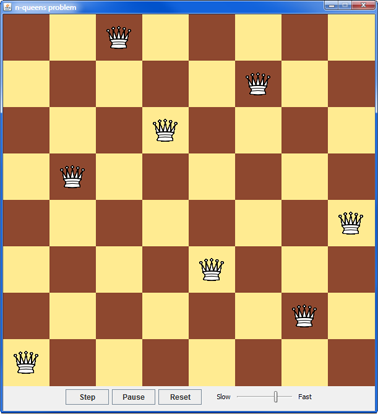
\includegraphics[scale=0.3]{img/8queens.png}
\caption{8 Queens Problems}
\end{figure}
\end{frame}

\begin{frame}[fragile]
\frametitle{8 Queens Problems}
{\tiny
\lstinputlisting{code/8queens/queenproblem.h}
}
\end{frame}

\begin{frame}[fragile]
\frametitle{8 Queens Problems}
{\tiny
\lstinputlisting{code/8queens/queenproblem.cpp}
}
\end{frame}

\begin{frame}[fragile]
\frametitle{8 Queens Problems}
{\tiny
\lstinputlisting{code/8queens/chessboard.h}
}
\end{frame}

\begin{frame}[fragile]
\frametitle{8 Queens Problems}
{\tiny
\lstinputlisting{code/8queens/main.cpp}
}
\end{frame}


